\documentclass[a4paper, 12pt]{article} 
\usepackage[top=2cm, bottom=2cm, left=2.5cm, right=2.5cm]{geometry}
\usepackage[utf8]{inputenc}
\usepackage{amsmath, amsfonts, amssymb}
\usepackage{graphicx} %pacote para inserir figuras
\usepackage{float} %força posicionamento da figura - para usar: subtituir [htb] por[H]
\usepackage[brazil]{babel} %força latex a escrever figura e não figure
\usepackage{lipsum} %para inserir textos lorem ipsum
\usepackage{subfig}
%\usepackage{setspace}

\begin{document}

\section{Inserindo Figuras lado a lado}

\begin{figure}[!htb] %tenta colocar here, depois top, depois bottom
	\centering %centraliza
	\label{FiguraTotal} %rotulo da figura
	\subfloat[Subfigura 1 \label{subfigura-1}]{ 
		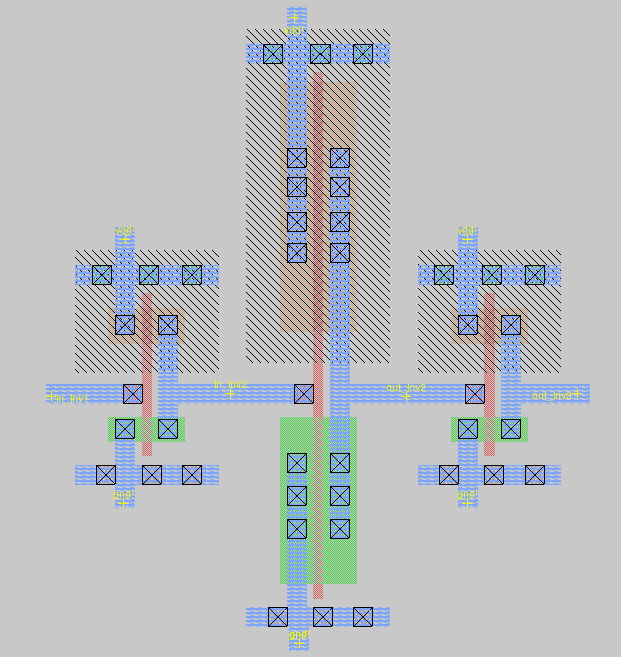
\includegraphics[width=0.48\textwidth]{images/inversores2.png} %width ou scale ou ...
	}\hfill
	\subfloat[Subfigura 2 \label{subfigura-2}]{ 
		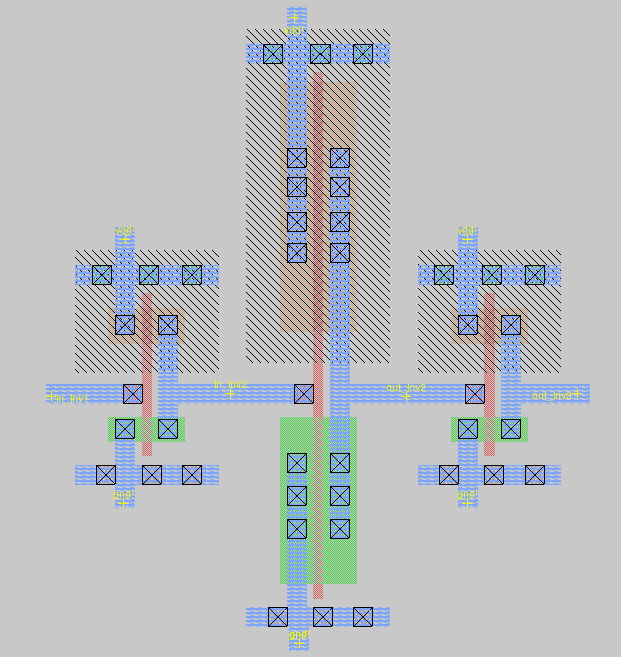
\includegraphics[width=0.48\textwidth]{images/inversores2.png}
	}
	\caption{Usando 2 figuras: \ref{subfigura-1} e \ref{subfigura-2} lado a lado com legenda} %legenda global das 2 figuras
\end{figure}


\end{document}